\chapter[Machine Learning in Gravitational wave Astronomy]{Machine Learning in Gravitational Wave Astronomy}\label{ch:chap_3}
% Brilliant catalogue of recent machine learning work
% https://iphysresearch.github.io/Survey4GWML/

%
% Introducing the chapter
%
It is expected that in the coming years the \ac{LIGO} detectors will see an increase in sensitivity. With this increase in sensitivity also comes an increase in the number of \ac{CBC} signals which will be detectable by the collaboration. The number of signals per year is expected to be anywhere on the order of 100s to 1000s (depending on the source type)~\cite{2018LRR....21....3A}. As such, it is imperative that we develop new techniques to deal with this massive influx of detectable sources. We also note that some signals and noise cannot be accurately modelled using traditional approaches, thus there is also a need to develope 
flexible tools to solve this problem. \ac{ML} has been proven to be an excellent resource for tackling many problems in the \ac{GW} community. Over the past several years, there has been a boon in the use of \ac{ML} methods across a variety of applications in detection, parameter estimation and detector characterization algorithms (among other domains). This surge in applications has seen marked success not only in proof-of-principle studies, but even in studies involving the use of actual \ac{LVK} data. Going forward, it is the hope of this author and surely other \ac{ML} \ac{GW} practitioners that after rigorous testing, these methods continue to be more widely used and for some, eventually implemented in realtime during observing runs in 
order to further enhance the capabilities of future \ac{GW} detectors.

In this chapter I will provide an overview of recent advances in \ac{ML} approaches in \ac{GW} astronomy in signal detection, parameter estimation, population inference and detector characterization.

\section{Machine Learning for Gravitational Wave Detection}

\ac{LVK} algorithms which search for \ac{GW}s are typically concerned with four types of sources: \ac{CBC}, Burst, \ac{CW} and stochastic \ac{GW}s 
(Sec.~\ref{sec:sources_methods}). 
\ac{CBC} sources being composed of \ac{BBH}, \ac{BNS} and 
\ac{NSBH} signals (Sec.~\ref{sec:CBC_source}), 
\ac{CW} sources composed of fast spinning \ac{NS}s (Sec.~\ref{sec:CW_source}), Burst are unmoddeled/poorly modeled signals like supernova or even as yet unknown sources (Sec.~\ref{subsec:burst_sig}), and stochastic \ac{GW}s result from left over remnants of the Big Bang along with poorly resolved \ac{CBC} signals from extreme distances (Sec.~\ref{sec:stochastic_source}). In this section we will outline several recent and interesting studies which have used \ac{ML} to directly 
detect \ac{GW}s from a variety of the aforementioned sources listed above.

%
% Seminal GW detection papers
%
\subsection{Compact Binary Coalescence Detection Studies}
Deep learning algorithms were first applied to the task of 
detecting simulated \ac{GW}s by 
George$\&$Heurta~\cite{PhysRevD.97.044039} and 
Gabbard \textit{et al.}~\cite{PhysRevLett.120.141103}. In our 
work (Ch.~\ref{ch:chap_4}), our \ac{ML} algorithm was trained 
on simulated \ac{BBH} waveforms in Gaussian noise and Gaussian 
noise alone\footnote{The noise generated was not white and was 
simulated from a realistic detector \ac{PSD}} to perform a 
classification task. Gaussian noise was used because it is 
known that matched filtering performs efficiently under 
Gaussian noise conditions~\cite{PhysRevD.49.2658} and 
Gaussian noise was a simple 
first step towards trying to match the efficiency of matched filtering. 
We note that it is known that matched filtering is not the 
optimal approach when searching over discrete 
waveform templates~\cite{2008arXiv0804.1161S,2021arXiv210403961Y} and 
\ac{ML} has in fact been 
shown to even exceed matched filtering sensitivity 
in some circumstances~\cite{2021arXiv210403961Y}. Using a \ac{CNN}, 
we were able to show that deep learning could match 
the efficiency of matched filtering. In ~\cite{PhysRevD.97.044039}, 
they also show that a similar \ac{CNN} approach 
(``deep filtering'') could reproduce predictions 
from matched filtering. In addition to signal detection, 
they were able to show that a \ac{CNN}, for the first time, could 
perform point-estimate parameter estimation on both 
\ac{BBH} and eccentric \ac{BBH} waveforms, 
closely matching the best-fitting templates predicted by 
matched filtering. It should be noted here that 
``close'' is a relative term if there are no uncertainties on those 
estimates. They 
additionally compare their \ac{ML} approach to other 
common \ac{ML} approaches including: K-nearest neighbor, 
support vector machines and logistic regression (among others) 
showing their \ac{CNN} to have superior results. 

%
% Discsussion on study differences between Gabbard and G&H
%
George$\&$Heurta use two network archetectures in their 
study: one for parameter estimation and one for signal 
detection. The parameter estimation network is composed of 4 convolutional 
layers, 4 max pooling layers, 1 flattening layer, 3 fully-connected 
layers and rectified linear unit activation functions on all 
fully-connected/convolutional layers, whereas the signal detection 
network is slightly smaller with 3 convolutional layers, 3 pooling 
layers, 1 flattening layer and 2 fully-connected. Gabbard~\textit{et al.} 
on the other hand used a slightly deeper network 
with 6 convolutional layers, 3 max pooling layers, 1 flatting 
layer, 2 fully-connected 
layers and exponential linear unit activation functions on all 
fully-connected/convolutional layers. In both studies, the number 
of filters in each convolutional layer increases up to the flattening 
layer, while conversely the kernel size decreases. The time to train 
both George$\&$Heurta networks was shown to be a few hours and 
evaluation of a single test sample took $\sim 6.7$ms for signal detection 
and $\sim 85$ms using the parameter estimation network. 
Gabbard~\textit{et al.}'s network took $\sim 1$ hour on a single 
\ac{GPU} and could produce signal detection statistics for a 
test sample on the order of milliseconds.

%
% Are CNNs a magic bullet Gebhardt paper
%
%There have been numerous follow-up studies which have explored the 
%use of \ac{ML} for \ac{CBC} detection. Gebhardt \textit{et al.} looked 
%into the feasibility of using \ac{CNN}s under more 
%realistic noise/signal conditions. They claimed in~\cite{1904.08693} 
%that \ac{CNN}s alone should not be used to describe the statistical 
%significance of a detection, but 
%rather are best suited as a realtime trigger generator to be 
%used for identifying events of interest for later study. Furthermore, 
%they state that a standard binary 
%classification approach does not necessarily indicate where precisely to 
%look in a time series window~\footnote{We note that this is not necessarily 
%a problem, as a simple regression will provide this to the same level of 
%accuracy as matched filtering.} for an event, which can be problematic 
%for follow-up analysis which require well localised \ac{GW} 
%triggers~\cite{0264-9381-33-21-215004}. 

%Additionally, they explain that 
%for a \ac{ML} binary classification scheme, the 
%\ac{FAR} is determined through a sliding 
%detection threshold value over a population of events, thus there 
%is only a single significance level produced for a given candidate 
%\ac{GW} event.~\hunter{I'm very confused by their statement here}.

%
% Their proposed solution to binary classification problems. 
%
%They propose a solution to some these issues by using a fully-convolutional 
%approach, where fully-convolutional means that every layer is entirely 
%made of convolutional filters. They claim that their 
%fully-convolutional approach is ideal 
%because the model makes minimal assumptions on the input data size and also 
%isolates the exact temporal location of a potential \ac{GW} candidate event 
%in a given timeseries. 
%The temporal location of an event is determined through the output of their 
%network which produces a single value between 0 and 1 for each element in a 
%given input time series. If a value is 1, that means it's likely that there is a 
%\ac{GW} signal present at that location, whereas 0 indicates 
%the presence of noise. The output values of their network are bounded between 
%0 and 1 through a sigmoid activation function. They were able to show that 
%their approach could successfully recover both real and 
%simulated \ac{GW} events in real detector noise.

%
% Gebhardt hypothetical signal discussion
%
%Gebhardt~\textit{et al.} perform additional tests on their approach, 
%using ideas from activation maximisation~\cite{10.1007/978-3-319-10590-1_53} and 
%adversarial attacks~\cite{2013arXiv1312.6199S}, and show that 
%their network may assign a high probability of a noise signal being 
%a \ac{GW} event, with only minor arbitrary changes to a noise-alone 
%timeseries. This is done by randomly selecting a noise-alone timeseries from 
%their test set, assigning a label of 1 over an interval in the middle of the %signal and 0 for all other portions of the signal. The noise-alone signal 
%is then given as input to a pre-trained network whose weights are fixed and 
%a loss is computed between the output of the network and the assigned labels 
%to the noise signal. The input is then updated through backpropogation of the 
%loss (network weights remain fixed), such that it minimises the loss. 
%This is then repeated for a number of iterations and the resulting input minus 
%the original input prior to backpropogation is thought of as a 
%noise signal which may fool the network into thinking a \ac{GW} is present. 
%They find that although many of these modified noise signals do have 
%chirp-like properties, there are a few concerning examples where the 
%signals do not have any \ac{GW}-like properties and 
%where the modified noise signal is only marginally different from the 
%original noise input signal, thus implyig that \ac{CNN}s may easily be fooled 
%by some plausible noise signals. As is mentioned in their manuscript, there is %still much study left to be done as to whether or not the examples used are too %contrived and not something we would realistically expect to see in the \ac{LVC} %detectors~\cite{1904.08693}.

%
% Harvard BNS paper
% https://www.sciencedirect.com/science/article/pii/S0370269320301349?via%3Dihub
It was first shown by Krastev~\textit{et al.}~\cite{KRASTEV2020135330} 
that using \ac{ANN}s one could accurately recover \ac{BNS} 
signals in Gaussian noise. The problem was posed as a 
trinary classification task whereby the \ac{ANN} model was tasked 
with distinguishing between \ac{BBH}, \ac{BNS} and Gaussian 
noise alone timeseries segments. Their neural network was 
limited to analysing data selected from a sliding window 
of $\sim10$s due to computational expense associated with 
analysing long timeseries segments. They also train their network 
through curriculum learning whereby the network is initially 
trained on easy-to-detect high \ac{SNR} signals and then gradually given 
more and more low \ac{SNR} signals as training progresses. Their results 
%using 
%\ac{ROC} curves~\cite{everitt2010cambridge}, a figure of merit 
%which denotes the ability of a method to classify events as 
%its discrimination threshold is varied, 
are quantified by comparing the \ac{TAP}, fraction of signals correctly 
identified and \ac{FAP} of predictions from their neural network classifier
for different classes of signal (i.e. \ac{BBH}, \ac{BNS}, noise-alone) 
(also known as a \ac{ROC} curve~\cite{everitt2010cambridge}). Their results 
show that that their network is more sensitive to detecting \ac{BBH} 
events than for \ac{BNS} events.
show that their \ac{ANN} 
performs more poorly on \ac{BNS} signals than on 
\ac{BBH} signals. To expand, $100\%$ of \ac{BBH} events 
are detected above an \ac{SNR} of 10, whereas $100\%$ of \ac{BNS} events 
are only detected above an \ac{SNR} of 18. They additionally quantify 
their results by plotting the \ac{TAP} as a function of \ac{SNR} at 
different \ac{FAP} values for both \ac{BBH} and \ac{BNS} neural 
network predictions. Their results for the \ac{BBH} case reach similar levels 
of sensitivity as those achived by 
Gabbard~\textit{et al.}~\cite{PhysRevLett.120.141103}. They state that 
the sensitivity difference between \ac{BNS} and \ac{BBH} neural network 
predictions could be due to a number of reasons including: 
sliding window size, network architecture choice and signal complexity. 
The authors do not compare their approach to any other 
existing currently used signal detection method such as 
matched filtering.

%
% Marlin BNS paper
% https://journals.aps.org/prd/abstract/10.1103/PhysRevD.102.063015
In Marlin \textit{et al.}~\cite{PhysRevD.102.063015}, 
the authors perform a more 
in-depth study on \ac{ML} for \ac{BNS} detection and use a different 
neural network architecture. In order to 
reduce the overall complexity of the input space they deal with 
32s long \ac{BNS} signals and vary the sample rate as a function of 
different segments in time of the signal. The authors justify this 
sampling approach by describing that most of the \ac{SNR} of the 
signal is contained in the final few seconds. Additionally, if one 
looks at the frequency evolution of a \ac{BNS} signal, we see that, for example,
at 16 s prior to merger for a 1.35-1.35 system, the GW frequency is 
48.7 Hz. Hence prior to this, a sampling frequency of at least 
100Hz would theoretically suffice. They state that using a 
varying sample rate also 
reduces the size of input signal space by a factor of $\sim 9$, thus 
decreasing the computational expense needed to run their 
approach. Their approach was also the first to probe \ac{ML}-based 
detection algorithm sensitivities down to \ac{FAR}s of about 0.5 per month. 
The authors also improve on previous architecture approaches by employing 
inception modules~\cite{1409.4842}, temporal convolutions for signal
amplification,~\cite{inproceedings_temporal} and tailoring 
inception modules for each different sampled section of 
the input time series~\cite{PhysRevD.102.063015}. Results from 
their study show an overall improvement in \ac{BNS} detection sensitivity 
with respect to results from Krastev~\textit{et al.}~\cite{KRASTEV2020135330}.
They quantify this by comparing results from their study with 
Krastev's study by plotting the \ac{TAP} as a function 
of \ac{SNR} for both studies. Marlin~\textit{et al.} are able to 
produce predictions with their neural network on a given input with a 
latency of $\sim10.2$s. The authors compare their results to 
traditional techniques like matched filtering 
(i.e. the PyCBC live event trigger 
generator~\cite{0264-9381-33-21-215004}) using a quantity known 
as the sensitivity distance~\cite{PhysRevD.102.063015} at fixed 
\ac{FAR}s. The authors find that their \ac{ML} approach has 
a sensitivity distance 
which is $\sim 6$ times lower than that of results from 
PyCBC at a \ac{FAR} of 0.6 per month. The authors also 
compare their results to Krastev~\textit{et al.}~\cite{KRASTEV2020135330} 
and see that for a given fixed \ac{FAR}, Marlin~\textit{et al.}'s 
network does not generalise well to high \ac{SNR} signals to the 
same sensitivity as Krastev~\textit{et al.}~\cite{KRASTEV2020135330} 
in terms of \ac{TAP} values. On the other hand, the results of 
Marlin~\textit{et al.} show a $\sim 4$ times increase in 
\ac{TAP} sensitivity 
over Krastev~\textit{et al.}~\cite{KRASTEV2020135330} in the lower 
\ac{SNR} regime ($8 \leq \mathrm{SNR} \leq 15$).
The authors mention that some general improvements 
could be made including: lowering the latency of their \ac{ML} 
approach by reducing 
the complexity of the network, the addition of real noise to the training/
testing sets, and using results form their approach as input 
to follow-up analysis by a traditional matched filtering algorithm with 
a heavily reduced template bank.

%
% CBC ML Honorable mentions paragraph
% 
We also note here that there are many other studies that have been done 
within the context of \ac{CBC} detection using \ac{ML} that we 
do not have the space to mention in this chapter. Some other notable 
examples include: using scalable autoencoders for \ac{CBC} \ac{GW} 
detection~\cite{CORIZZO2020113378}, genetic-algorithm-optimized neural 
networks for \ac{CBC} \ac{GW} detection~\cite{2020arXiv201004340D}, using 
\ac{CNN}s given time-frequency input representations to detect \ac{CBC} 
\ac{GW}s~\cite{9412180},  and detecting the early insprial of \ac{CBC} \ac{GW} 
signals using \ac{CNN}s~\cite{2021arXiv210513664B}. We will now 
discuss how \ac{ML} is being applied towards the detection 
of burst \ac{GW} signals.

%
% Burst detection papers
%
\subsection{Burst Detection Studies}

%
% First implementation of Burst machine learning paper
% 
The first implementation of a machine learning algorithm for the 
purpose of identifying burst-like signals was by Astone~\textit{et al.} 
in 2018~\cite{2018PhRvD..98l2002A}. In their paper they 
build upon the already existing \ac{CWB} pipeline~\cite{PhysRevD.72.122002} 
used by the \ac{LVC}. Specifically, they are interested in 
searching for core-collapse supernovae
events~\cite{Ott_2009}. Their method can be 
summarised in two steps. First, they prepare time-frequency 
images of detector data using the \ac{CWB} event trigger generator,
which searches 
for periods of excess power and combines these 
periods coherently among the various detectors (for further 
details on coherent searches see 
either Ch.~\ref{ch:chap_1} or \cite{PhysRevD.72.122002}).
Once periods of excess power have been identified, a time-frequency 
spectrogram image is constructed for each active detector. 
In their approach, they use three detectors and 
combine them in such a way that each detector essentially acts as a colour
channel, akin to a red-green-blue (RBG) colour scheme. The authors then 
use a \ac{CNN} to classify the identified time-frequency image into 
either noise or signal+noise classes. They test their network on a 
range of signals spanning \ac{SNR} values from 8 up to $\sim 40$. They 
show that their method is overall more efficient at detecting 
core-collapse supernovae signals than the standard detection pipeline \ac{CWB} at a \ac{FAR} of around $7 \times 10^{-7}$.

%
% Other studies which use ML for burst detection (in brief)
% 
It was also shown in Chan~\textit{et al.}~\cite{PhysRevD.102.043022}, 
that \ac{CNN}s may be used to detect \ac{GW}s resulting from 
core collapse supernovae events. In their work they find that 
their approach would be able to detect core collapse supernovae 
events out to a distance of 60kpc with a \ac{TAP} of $\sim 54\%$ 
at a \ac{FAP} of $0.1\%$, well withing the distance to the large and 
small Magellenic clouds. Additionally, 
McGinn~\textit{et al.}~\cite{2021CQGra..38o5005M} 
applied a \ac{ML} algorithm known as a \ac{GAN}~\cite{1406.2661} 
in order to produce generalised 
\ac{GW} burst waveforms in the time domain. Their network was trained 
over 5 different classes of waveforms commonly used by burst searches 
and find that, once trained, their \ac{GAN} model is able to 
accurately produce waveforms on-command which are similar in waveform 
characteristics those it was trained over, as well as generalise to 
other waveforms which act as hybrids between the 5 training classes. 
They test the practical aspects of their work by first training a \ac{CNN} 
solely using the 5 well-defined classes of waveforms used by their 
\ac{GAN} during training and then training another identical \ac{CNN} 
using a training set which is generated using waveform timeseries produced 
by their \ac{GAN}. The authors find that the \ac{CNN} trained with 
waveforms generated by the \ac{GAN} had superior performance over 
the \ac{CNN} trained with the 5 classes alone and quantify this 
through efficiency curves which measure the \ac{TAP} as a function 
of \ac{SNR} at fixed \ac{FAP} values.

%
% Final paper 
%
Finally, we note the recent study by 
Vaselios~\textit{et al.}~\cite{2020arXiv200914611S} 
which showed for the first time that a multi-component \ac{CNN} architecture 
was able to classify unmoddeled bust signals. They train their model 
using white-noise burst signals~\cite{Sutton_2010} buried in Gaussian noise 
and Gaussian noise-alone timeseries. Their network architecture is unique 
in that it employs two \ac{CNN}s: one for identifying signals which are 
coincident between detectors and the other for detecting correlations 
between detectors. The first \ac{CNN} was derived from the same architecture 
as Gabbard~\textit{et al.}~\cite{PhysRevLett.120.141103} 
and is given as input a timeseries and 
produces an output between 0 and 1, denoting the likelihood of the timeseries 
containing either a signal or noise respectively. The second network takes 
as input again a timeseries, but is also given the 
Pearson correlation~\cite{2020arXiv200914611S} for each pair of detectors 
and outputs values between 0 and 1, 
where 0 indicates low correlation and 1 indicates high correlation between detectors. This dual \ac{CNN} setup is inspired by the operation of 
standard burst \ac{GW} detection pipelines which require that a signal 
is both coincident and correlated between
detectors~\cite{2020arXiv200914611S}. They test their 
method under a variety of waveform morphologies and illustrate their 
sensitivities through computing \ac{TAP} values at fixed \ac{FAP}s across 
a range of \ac{SNR} values. In the next section, we will discuss how 
\ac{ML} has been applied to the search \ac{CW} signals.

%
% CW detection papers
%
\subsection{Continuous Wave Detection Studies}

%
% First CW ML paper
% https://journals.aps.org/prd/pdf/10.1103/PhysRevD.100.044009
In terms of \ac{CW} searches, the standard amount of time taken to 
perform coherent or semicoherent searches can be computationally 
expensive, sometimes taking well over a month to 
complete~\cite{PhysRevD.100.044009}. Dreissigacker~\textit{et
al.}~\cite{PhysRevD.100.044009} try to decrease 
this computational time with respect to standard \ac{CW} detection 
approaches using ResNet neural
networks~\cite{2015arXiv151203385H} in the first application of 
deep learning for the \ac{CW} search. They frame the problem 
such that their training set consists of two types of input. One, 
being long $10^6$s signals and shorter $10^5$s signals. Rather than 
doing a search over the entire frequency range, they limit their 
test cases to a discrete set of frequency bands, $50$mHz 
in width, at (20, 100, 200, 500 and 1000 Hz). They compare their 
\ac{ML} results to a ``gold standard'' \ac{CW} search method 
pipeline \texttt{WEAVE}. The pipeline sums 
coherent $F$-statistics~\cite{1998PhRvD..58f3001J} over 
semicoherent segments~\cite{PhysRevD.90.122010}
on lattice-based \ac{GW} template
banks~\cite{2007CQGra..24S.481P}, although their study 
employs the fully coherent search version of the 
code. The reason there is both a semicoherent and a fully coherent 
version of the \texttt{WEAVE} code is related to the computational 
cost of performing a fully coherent search. Given that \ac{CW} signals 
are weak in amplitude, one needs to analyse long periods of data 
in order to accumulate enough \ac{SNR} to make a detection. However, 
the computational expense of performing the optimal fully coherent search 
scales as $T^n$ where $T$ is the length of the data analysed 
(this 
is especially problematic at high 
frequencies~\cite{PhysRevD.90.122010}). Semicoherent 
methods for performing a \ac{CW} search were thus developed with the purpose 
of making it possible to analyse longer stretches of data with reduced 
computational cost.

%
% More info on first CW ML detection paper
%
For the training set, Dreissigacker~\textit{et
al.} generate over $10^4$ training waveforms in the frequency 
domain with half containing 
Gaussian noise and the other half containing signal+noise. 
They found that using a set greater than $10^4$ training signals 
provided little gain in 
efficiency. After training, the authors found that at a fixed 
\ac{FAP}, their deep learning approach appears to be 
competitive ($88 - 73\%$ detection probability) with the matched 
filtering search ($\sim90\%$ detection probability) on short time 
scale inputs ($10^5$s). However, when tasked with longer time scale 
inputs ($10^6$s), the neural network performs at a diminished 
detection probability ($69-13\%$). 
In terms of computational speed, it was also shown that 
their neural network outperformed the matched template search, 
taking only on the order of a few 
milliseconds ($3 - 10$ms) as opposed to the $10^6 - 10^9$s of the 
matched filter method. The authors do also note however that the network 
requires $\sim 1 - 10$ days to train depending on the length of the 
observed data, $T$, used. As the authors state, there 
is much work to be done in order to improve
the efficiency of deep neural networks within the context 
of \ac{CW} searches. There is also much promise given the quality 
of results achieved thus far. In a follow-up to~\cite{PhysRevD.100.044009},
Dreissigacker~\textit{et al.} show in~\cite{2020PhRvD.102b2005D} 
that using an Inception-ResNet~\cite{2016arXiv160207261S} 
architecture they were able to 
train a deep neural network to classify the presence of \ac{CW} signals 
given data from 2 detectors simultaneously. They also showed that their 
network code was able to show an approximately equivalent sensitivities 
under both targeted search and all-sky search \ac{CW} scenarios. We also 
note the recent \ac{ML} \ac{CW} studies 
cited here~\cite{2019arXiv190706917M,2020past.conf...33M}.


\section{Machine Learning for Gravitational Wave Bayesian Parameter Estimation}

%
% Intro
%
For many, \ac{GW} parameter estimation was the ``holy grail'' of machine learning in the field of \ac{GW} astronomy. Although prior to 
2019 there were some attempts to compute point estimates for 
\ac{GW} source parameters directly, as well as to incorporate 
\ac{ANN}s directly into subsections of existing Bayesian inference 
algorithms~\cite{10.1111/j.1365-2966.2011.20288.x}, there had up to 
that point been no studies done using an \ac{ML} algorithm which went 
from directly from strain to computing samples from the Bayesian posterior 
on \ac{GW} source parameters. In this subsection, we will outline 
some recent studies on incorporating \ac{AI} into existing 
\ac{GW} parameter estimation pipelines, \ac{ML} for 
point estimate parameter estimation and finally \ac{ML} for 
directly computing samples from the Bayesian posterior.

%
% Beginnings BAMBI and point estimate PE
% BAMBI: https://academic.oup.com/mnras/article/421/1/169/989639
\ac{ML} was first used in the context of \ac{GW} parameter 
estimation by Graff~\textit{et al.}~\cite{10.1111/j.1365-2966.2011.20288.x}
in their modified nested sampling algorithm \texttt{BAMBI}. 
In their algorithm, the authors exploit the tenants of the 
universal approximation theorem~\cite{HORNIK1990551}, which implies 
that even a properly optimized \ac{ANN} should be able to 
approximate any sufficiently complicated likelihood function. 
This is done by essentially replacing the computationally 
expensive likelihood calculation 
in the \texttt{MultiNest}~\cite{2009MNRAS.398.1601F} nested 
sampling algorithm (Sec.~\ref{sec:nested_sampling}). After the 
nested sampling algorithm has produced a sufficient number of 
samples, their \ac{ANN} is trained on those samples. The inputs 
to the \ac{ANN} are the sample parameter values 
and the output is a single scalar which represents the likelihood 
values for each of those samples. The \ac{ANN} is then trained 
such that it's predictions for the likelihood values match 
those computed within the nested sampling algorithm. The advantage 
of having such a \ac{ANN} is that once trained, the \ac{ANN} can 
provide near instantaneous likelihood evaluations. In order to 
quantify when the \ac{ANN} has been trained sufficiently to 
fully replace the standard likelihood function, a tolerance level 
is calculated. The tolerance is defined as the standard 
deviation of the difference between the true log-likelihood 
values from nested sampling and the predicted values from the 
\ac{ANN}. The actual value of this tolerance level may 
be specified by the user. Once the network has 
reached an acceptable tolerance level of performance it 
then replaces the original likelihood function calculation. 
Periodic tolerance checks are made throughout the rest of the 
nested sampling iterations to ensure that the \ac{ANN} is still 
providing solid predictions.

The authors find that their algorithm performs well across a variety 
of toy model cases (Gaussian shells, Rosenbrock
functions~\cite{Shang2006ANO}, 
eggbox~\cite{2009MNRAS.398.1601F}). They also compare their 
approach (\texttt{BAMBI}) to unmodified \texttt{MultiNest} on a 
few real physics examples including predicting the posteriors of 
8 cosmological parameters using data from \ac{CMB} observations 
and \ac{CMB} observations plus Hubble Space Telescope constraints 
on $H_0$, the Sloan Digital Sky Survey and Type 1a Supernovae data 
(see~\cite{10.1111/j.1365-2966.2011.20288.x} for more details 
on datasets used). 
The gain in speed goes from taking on the order of seconds per 
likelihood calculation, down to milliseconds, a three order of 
magnitude increase in computational performance with 
accurate evidence predictions and posterior 
probability distributions~\cite{10.1111/j.1365-2966.2011.20288.x}.

%
% Your paper on Bayesian PE
%
One of the first implementations to use a purely \ac{ML}-based 
algorithm to produce Bayesian posteriors was performed 
by Gabbard~\textit{et al.} 
in~\cite{1909.06296}. In our study (also discussed in heavy detail in 
Ch.~\ref{ch:chap_4}), we show that using a \ac{CVAE}, given a timeseries, 
we can produce Bayesian posteriors over the full \ac{GW} 
\ac{BBH} parameter space. 
The network is trained over \ac{BBH} \ac{GW} waveforms in Gaussian noise, 
as well as the source parameters which characterise the \ac{BBH} waveforms. 
Once trained, our network can produce $\sim 8000$ posterior samples 
per given timeseries in $\sim 0.1$ms. We compare our results against 
four benchmark Bayesian samplers (\texttt{Dynesty}, \texttt{ptemcee}, 
\texttt{emcee}, \texttt{CPNest}) and find that our \ac{ML} model is 
generally consistent with other benchmark approaches. Consistency 
is quantified through a combination of \ac{JS}-divergence and \ac{PP} 
plot tests, as further outlined in Ch.~\ref{ch:chap_4}.

%
% Alvin Chua paper
% 
Released at the same time as Gabbard~\textit{et al.}~\cite{1909.06296}, 
Chua \textit{et al.}~\cite{2019arXiv190905966C} also aimed to show that 
\ac{ML} methods could accurately 
approximate Bayesian \ac{GW} posteriors. Their method used 
fully-connected neural networks (Ch.~\ref{ch:chap_2}). They represent 
their training waveforms by first training a neural network to 
predict coefficients which describe a reduced order
framework~\cite{PhysRevLett.122.211101}. Once trained, the 
network is able to quickly produce training \ac{GW} waveforms. 
Their training \ac{GW} waveforms are represented in 
the frequency domain, whereby there are both real and imaginary 
components of the wavefrom. The authors use  
two networks which produce the real and imaginary components of the 
waveform separately. To produce posteriors, 
Chua~\textit{et al.} again use a fully-connected neural 
network which takes as input during training the 
training waveforms (in Gaussian noise), as well as the source 
parameter values of those training waveforms. Their model then outputs 
a $1-$ or $2-$dimensional posterior in the form of a multivariate 
Gaussian whose means and covariance matrix are predicted by 
the neural network. When testing, the model is constructed such that 
it only needs as input the test sample waveform alone. One can then 
produce samples from the posterior for a given input waveform by 
sampling from the predicted multivariate Gaussian. 
\hunter{I could try to explain the loss, but that part of the paper is uninterpretable to me.}
%and 5 values which 
%parameterise a bivariate Gaussian distribution. 
%The loss function is the cross entropy between the 
%natural log of samples from the predicted bivariate Gaussian and the training 
%waveform source parameter values.~\chris{you can only take the cross entropy %between 2 distributions so how do they do that for a histogram (which represents %a distribution) and a true source parameter value?} \hunter{I need help 
%explaining this.}

Chua \textit{et al.}~\cite{2019arXiv190905966C} test and 
train their model on \ac{BBH} waveforms, expected to be seen  
by space-based detectors such as \ac{LISA}, in Gaussian 
noise with masses ranging 
from $1.5 \times 10^5 - 10 \times 10^5$ with aligned spins 
between $-1$ and $1$. They then train their 
model to predict both the chirp mass and the symmetric mass ratio 
. Their results show good agreement between the posteriors 
produced by their machine learning approach and traditional 
Bayesian sampling 
approaches~\cite{2019arXiv190905966C,PhysRevLett.122.211101}. They 
more formally quantify the accuracy of their results by computing 
the sample covariance matrix of the posterior predicted by 
their neural network, as well as the covariance matrix of the 
true Bayesian posterior and then comparing both through a log ratio 
expression given in Eq.~9 of~\cite{2019arXiv190905966C}.

%
% Greeen 1st paper
%
Following on from Chua~\textit{et al.}~\cite{2019arXiv190905966C} and 
Gabbard~\textit{et al.}~\cite{1909.06296}, 
Green~\textit{et al.}~\cite{PhysRevD.102.104057} wanted to 
tackle two outstanding problems which both Chua \textit{et al.} and 
Gabbard \textit{et al.} had yet to solve at the time. With regards 
to Chua \textit{et al.}'s approach, it was to expand upon the 
limited number of source parameter dimensions that their algorithm 
could produce posteriors on at a time (no more than 2). With 
regards to Gabbard \textit{et al.}, it was the initial 
difficulty of dealing with multi-modal 
posteriors (which was later rectified in subsequent 
updates to our paper). In Green~\textit{et al.}'s first 
paper~\cite{PhysRevD.102.104057}, 
they implemented a new \ac{ML} approach using a combination of 
normalising flows~\cite{2015arXiv150505770J} and 
\ac{CVAE}s (Ch.~\ref{ch:chap_2}). 

A normalising flow  
% MAF citation ~\cite{2017arXiv170507057P} 
is a mechanism for mapping simple distributions to more 
complex distributions through a seris of transformations, 
while also retaining the property of being 
invertible. Invertibility 
meaning that in order to sample from the complex distribution, we must 
also still be able to sample from the simple distribution. As stated 
in~\cite{2015arXiv150505770J}, 
a normalising flow may in fact be represented as a neural network where 
the parameters which characterise the series of transformations in a 
flow, are learned by the neural network over the course of
training~\cite{Cuoco_2020}.
%This is done in practice by having a neural network predict mean and standard 
%deviation values describing Gaussian distributions, given random samples 
%from a more simple distribution (say a mean zero, unit variate Gaussian).
%Samples from a complex distribution may then be sampled by 
%computing the determinant of an inverse 
%Jacobian\hunter{I'm very confused about this ...}. 

In their paper, Green~\textit{et al.} use three distinctly 
different models to produce Bayesian posteriors: 
a \ac{CVAE}, a \ac{MAF}~\cite{2017arXiv170507057P} and a combination of a 
\ac{CVAE} and a \ac{MAF}.
The combined \ac{CVAE}+\ac{MAF} 
network, is constructed by appending flows to the 
end of both encoders and the decoder network of 
the \ac{CVAE} in order to better model more complex distributions 
in the latent space of the \ac{CVAE}. 
The authors test their methods on 1~s long \ac{BBH} signals in 
Gaussian noise sampled at 1024Hz and try to predict a 5 parameter case 
($m_1,m_2,\phi,t_0,d_\mathrm{L}$) and an eight 
dimensional case ($m_1,m_2,\phi,t_0,d_\mathrm{L},\chi_1,\chi_2,\iota$) 
which uses an aligned spin model. Both 
of these cases are using a single detector with fixed sky 
location. Prior to training, they perform a unique pre-processing 
step whereby they transform their training samples (
\ac{GW} waveforms in Gaussian noise) via principal component analysis 
into 100 element 
long series of principal components, thereby 
reducing the dimensionality of the input and 
vastly improving the overall computational cost of 
training/testing their network. 
They find that all three methods perform 
reasonably 
well, although the basic \ac{CVAE} alone method is not able to 
resolve the multi-modal source parameters such 
as phase. They validate their results quantitatively through a combination 
of \ac{PP} tests and computing the \ac{KL} divergence between mulit-
dimensional posterior 
distributions from their \ac{ML} approaches and those from a benchmark 
Bayesian sampler, \texttt{emcee}, with \ac{KL} values of 
$\sim 0.3$. For context they also computed the \ac{KL} divergence between 
samples which are drawn from identical posteriors and found that value to be 
$\sim 0.1$.

%
% Green second paper
%
In a subsequent paper, 
Green~\textit{et al.}~\cite{2008.03312} used a pure \ac{MAF} flow 
network with spline couplings~\cite{2019arXiv190604032D}. The authors 
train their model and then test on a known \ac{GW} signal in 
Gaussian noise (GW150914~\cite{PhysRevLett.116.061102}). 
After training, they 
find that their approach is able to to closely match a standard 
Bayesian sampler (\texttt{Dynesty}~\cite{dynesty}), according to corner plots, 
\ac{JS}-divergence values and \ac{PP} plot tests. They find  
minor inaccuracies on the inclination angle, where their 
\ac{ML} approach puts more imbalance in the posterior on one of the 
two modes in the posterior space.  

%
%Michael Williams Nessai
%
Using normalizing flows, 
Williams~\textit{et al.}~\cite{PhysRevD.103.103006} were able to replace 
the computationally costly task of drawing samples from the prior 
constrained by the likelihood contour of the lowest (worst) 
live point in an existing 
nested sampling algorithm with flows. The flow tries to model 
the multi-dimensional multi-modal likelihood contour defined by the worst live 
point. Their algorithm, dubbed \ac{NESSAI}, uses a 
specific type of flow, coupling flows, 
because of their computational cheapness (although with the 
added disadvantage of tending to be slightly less flexible 
than autoregressive flows). The flow is trained on the current set 
of live points through a loss function defined in Appendix A
of~\cite{PhysRevD.103.103006}. Once trained, the flow is then 
used to generate a population of new proposal points. A point is randomly 
drawn from this proposal population and its likelihood is calculated. 
The proposed point replaces the old worst live point 
if the proposed point likelihood is greater than the worst 
live point likelihood. This process is repeated until one of a number of 
criteria are met: the proposal 
population generated is depleted, acceptance rate of points drawn 
from proposal population is too low, a pre-determined number of new 
live points have been accepted, some user-defined nested sampling 
convergence threshold is passed. This is all further outlined in Sec. 3B 
of~\cite{PhysRevD.103.103006}. The authors find that when compared 
to the Bayesian sampler \texttt{Dynesty}, their approach is between 
$\sim 2.32$ and $\sim 1.40$ times faster depending on whether or 
not distance marginalisation is applied.
The majority of the computational cost of the \ac{NESSAI} algorithm is 
expended through the proposal population generation stage 
($36\%$ of the total cost for a given injection), while flow 
training only accounts for a small percentage ($9\%$). The proposal point
likelihood evaluation stage cost decreases as the number of 
CPU threads used in the analysis 
increases, falling to approximately $9\%$ of the total cost when using 
16 threads. \hunter{May want Chris to double check this.}

%
% Honorable mentions paragraph
%
We also mention that there are many other works in \ac{ML} 
for Bayesian parameter estimation which we do not have the 
space to discuss in more detail here. We highlight a few 
additional studies where for example it was shown that \acp{CNN} could 
be used to model the likelihood-to-evidence ratio in 
an \ac{MCMC} sampling algorithm~\cite{2020arXiv201012931D}. It was demonstrated 
in~\cite{2021arXiv210710730K} that a \ac{CVAE} (using a similar scheme 
as Gabbard~\textit{et al.}~\cite{1909.06296}) could be trained by 
also conditioning on the \ac{ASD}, thus allowing their network to generalise 
to a time varrying \ac{ASD}. Finally, it was also illustrated
in~\cite{2021CQGra..38o5010A} that 
a cross-residual network~\cite{2018arXiv181201187H}, 
given spectrogram data, could produce 
probability distribution of estimates on \ac{GW} source parameters~\footnote{
We note that the probability distribution generated is not a Bayesian 
posterior, but rather a distribution which models the uncertainty due to 
the stochastic processes of the neural network itself. This is done 
through a process known as Monte Carlo Dropout~\cite{2015arXiv150602142G}}. 
We will now discuss in the next section some new work on 
using \ac{ML} for \ac{GW} population inference.

\section{Machine Learning for Population Inference}

%
% Intro
%
Given the recent accumulation of \ac{GW} detections over the 
past several \ac{LVC} observation runs, we are now able to 
perform more detailed studies across a population of 
\ac{GW} events. It is also expected that as detector 
upgrades are made and new detectors come online, that we will start to 
see hundreds to thousands of \ac{GW} events per
year~\cite{2018LRR....21....3A}. Such abundance of signals will 
only enhance population studies which aid us in understanding 
\ac{GW} source formation channels, the general properties of \ac{GW} 
source parameters  (masses, redshifts, spins etc.), progenitor 
merger rates, as well as possible modifications of
\ac{GR}~\cite{Abbott_2019}. In order to constrain certain 
phenomenological models, it is common to employ the use of 
Bayes factors (Ch.~\ref{ch:chap_1}) comparing different model assumptions.
Employing such Bayes factors commonly involves the production of 
computationally costly simulations of synthetic populations 
of \ac{GW} events and then comparing those synthetic populations to 
real-world data~\cite{Zevin_2017}. One way of circumventing this 
is through \ac{ML}. 

%
% Wong first normalizing flow paper
%
Wong \textit{et al.}~\cite{PhysRevD.101.123005} showed for the 
first time that a hybrid normalizing flow---hierarchical Bayesian model 
framework was able to accurately 
constrain \ac{GW} population models~\cite{PhysRevD.101.123005}.
Specifically, the authors try to get a normalising flow to estimate 
the population likelihood, $p(\bm{\theta}|\bm{\lambda})$ (See Eq.~1 
in~\cite{PhysRevD.101.123005}), where $\bm{\lambda}$ 
are a set of hyperparameters which describe the general properties of
a set of \ac{GW} events. 
$\bm{\theta}$ in this case represents parameters 
which characterise single \ac{GW} events from the \ac{GW} event set. $p(\bm{\theta}|\bm{\lambda})$ is needed in order to calculate the 
likelihood of observing a particular set of \ac{GW} events
given population hyperparameters $p(\bm{d}|\bm{\lambda})$ (See Eq.~1 
of~\cite{PhysRevD.101.123005}) through 
hierarchical Bayesian model 
selection. \hunter{this whole paragraph up to here needs to be double 
checked.}
Their normalising flow is given as input 
parameters $\bm{\theta}$ and $\bm{\lambda}$ 
which characterise simulated \ac{GW} event catalogue sets and produces 
as output the population likelihood $p(\bm{\theta}|\bm{\lambda})$. 
Wong~\textit{et al.} show that their technique performs well 
over what were once considered highly intractable models. They compare 
their results to simulations using an analytic phenomenological 
model, which provides an exact analytic expression for
$p(\bm{\theta}|\bm{\lambda})$ which they can directly compare their predictions
of $p(\bm{\theta}|\bm{\lambda})$ form the normalising flow against. 
Although the authors neglect to take into account event 
uncertainties and selection bias, their \ac{ML} technique 
is shown to scale well, with up to 3000 \ac{GW} events in a set 
characterised by 6 \ac{GW} event parameters $\bm{\theta}$ and 
4 population hyperparameters $\bm{\lambda}$, producing 100 samples from 
$p(\bm{\theta}|\bm{\lambda})$ in 
$\sim0.1$s. Given that their model performs just as efficiently 
as other analytic approaches in a fraction of the time, it is 
likely that normalizing flows will play a crucial role in testing 
different state of the art models and even families of models 
in future \ac{GW} event catalogue releases. As is the case with 
most \ac{ML} approaches, more data and greater \ac{ML} 
model complexity may also improve results. We will now 
discuss in the next section how \ac{ML} has been 
used for the purposes of identifying and characterising 
non-astrophysical noise transients and glitches.

\section{Machine Learning for Detector Characterisation}

%
% Intro
% Would be nice to have fig of glitch in here somewhere
Non-astrophysical noise sources can affect the data quality of the 
detectors adversely. Poor data quality can not only be a 
source of confusion when doing data analysis, but can even entirely 
corrupt segments of data. It is the job of 
detector characterisation experts to identify and mitigate 
such noise disturbances. If we are able to identify and 
prioritize classes of glitches (non-astrophysical transients), this 
is an important first step in mitigating such events. In this 
subsection I will describe some recent efforts to use \ac{ML} to 
identify and mitigate noise in the \ac{LVK} detectors.

%
% Gravity spy
% Maybe have a plot of a glitch
In order to better classify known and unknown classes of glitches, 
Zevin~\textit{et al.}~\cite{0264-9381-34-6-064003} use a 
unique combination of human learning and \ac{ML} in a pipeline called
\texttt{Gravity Spy}. In \texttt{Gravity Spy} a set of glitch 
triggers are chosen for training which occur in ``lock'' 
(meaning the detector was in a proper state to search for 
\ac{GW}s, i.e. a state when it's sensitive for \ac{GW}s). The 
glitches themselves are represented through Omega
scans~\cite{Chatterji_2004}, 
which essentially search over sine-Gaussian waveform templates 
characterised by Q(quality) factor. Each template is represented as a time-frequency tiling and the Omega scan searches for templates 
which most closely match a given piece of data where a good match 
is defined as having a high \ac{SNR} value of the data with the template. A
time-frequency spectrogram is finally generated for the most 
significant tile of the best matching template. See 
Fig.~\ref{fig:gravity_spy_glitch} for an example of some glitches  
represented as Omega scans. 

%
% Gravity spy glitch figure
%
\begin{figure}
    \centering
    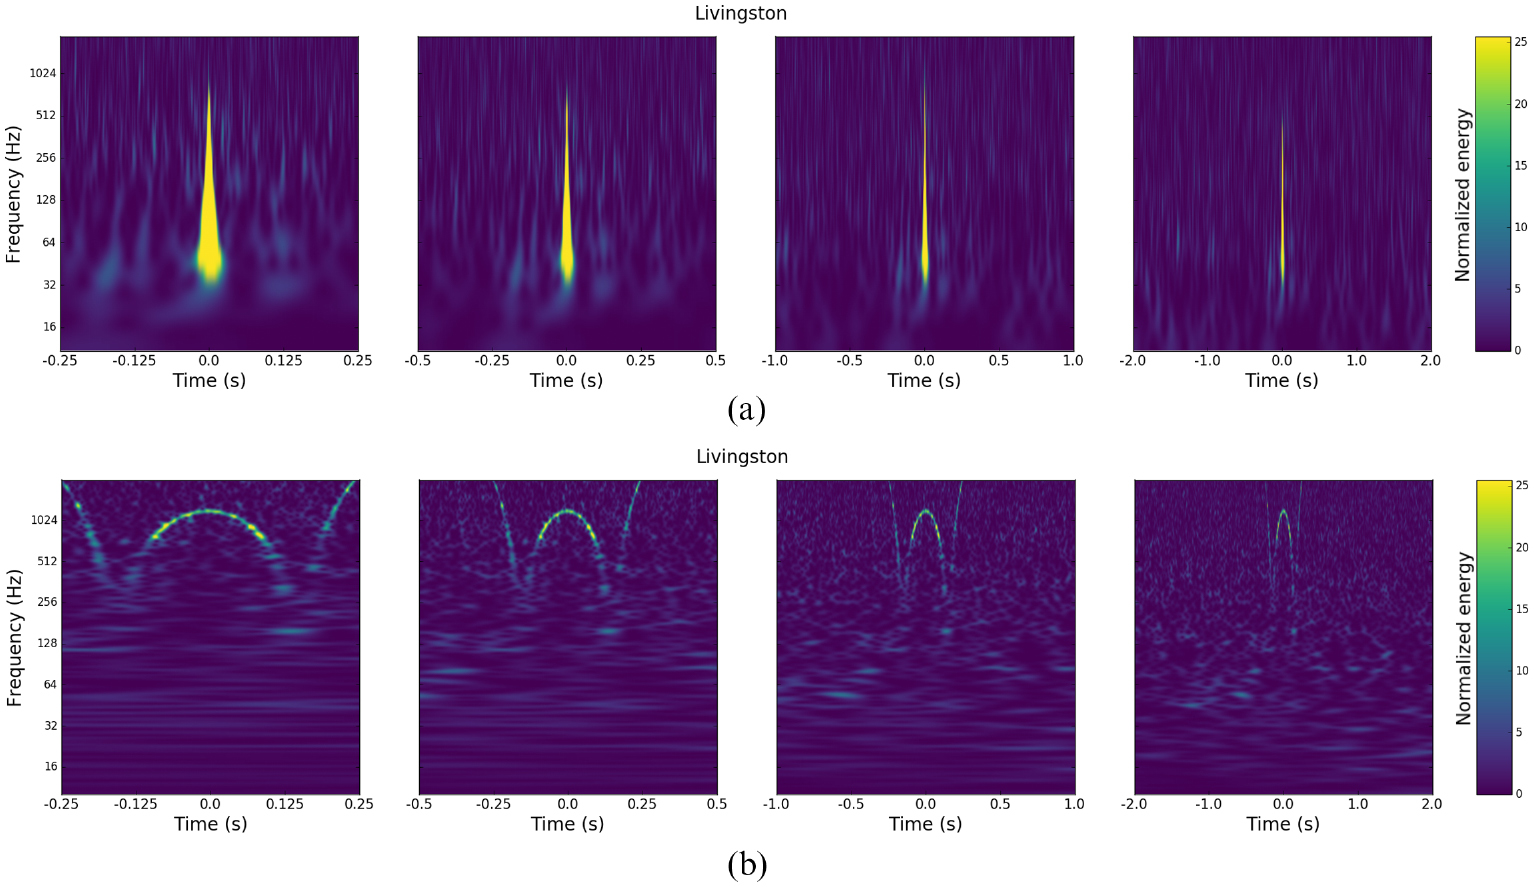
\includegraphics[width=\linewidth]{figures/gravity_spy_glitches.jpeg}
    \caption[An example of two glitches commonly identified by Gravity Spy 
    (blip and whistle)]{ In this figure we see examples of two glitch types 
    commonly identified by Gravity Spy. The top panels show a blip glitch in the 
    time-frequency plane at 4 different time windows 
    and is colorised by the normalised energy, which is 
    essentially a measure of loudness. The bottom panels are an example of a 
    whistle glitch, again at 4 different time windows. This figure was produced by the authors of \cite{0264-9381-34-6-064003}.}
    \label{fig:gravity_spy_glitch}
\end{figure}

%
% Gravity spy training
%
Their initial training set was generated from a set of $10^5$ Omicron 
glitch triggers, from which about $100$ glitches per class were 
identified by eye from trained detector characterization experts. 
Approximately $20$ classes were identified, where each were characterised 
by their corresponding waveform morphology. These $100 \times 20$
``gold-standard'' glitches were then used to train a preliminary neural 
network (a basic deep \ac{CNN} model (Ch.~\ref{ch:chap_2})) to 
identify the remaining glitches in the rest of the $10^5$ Omicron triggers. 
These triggers are then uploaded to the Zooniverse 
website~\cite{zooniverse.org} where volunteer citizen scientists are 
able to try classifying the trigger spectrograms by eye. Volunteers are 
initially trained on ``gold standard'' glitch images and other well known 
glitches which have a high probability of belonging to a specific class. 
After successive successful classifications by volunteers, the 
difficulty of glitches presented to the volunteers is ramped up. If a 
glitch is identified enough times by both the \ac{ML} algorithm and 
volunteers to a high degree of confidence, it is then ``retired'' 
whereby it is taken out of the volunteer glitch lookup pool and then 
added to the \ac{ML} labeled training set to improve the accuracy 
of the \ac{ML} model.

%
% Gravity results and take home message
%
Overall, \texttt{Gravity Spy} has been an incredibly successful use of \ac{ML} and a unique example of use citizen scientists for great gain. 
In addition, \texttt{Gravity Spy} is an excellent 
example of outreach which energises the 
general public to get more interested in \ac{GW} astronomy. Citizen 
scientists were able to identify more than $45,000$ glitches and 
several new glitch classes such as ``Paired Doves'' and 
``Helix'' glitches. The ``Paired Doves'' class 
was a particularly useful identification as it closely 
resembled that of a company binary inspiral signals, which means 
that it was a particularly problematic glitch type, since it mimics 
the general structure of a known \ac{GW} waveform. 

%
% Intro to genetic algorithms
%
One of the downsides of many \ac{ML} algorithms (and a topic this 
author is personally very interested in) is the idea of interpretability. 
Many \ac{ML} models such as \ac{CNN}s, \ac{GAN}s, \ac{CVAE}s, etc. 
while powerful are composed of millions of model parameters which 
interact in complicated non-linear ways. Trying to interpret \emp{why} a 
particular network configuration works over another is an active area of 
ongoing research in the \ac{ML} community. Genetic algorithms are unique 
in that they are more easily interpretable than many other approaches.

%A genetic algorithm is similar to a 
%decision tree~\cite{Kaminski2018}, where a decision tree is made up 
%of three components: nodes, branches and leaves. Nodes are representative of 
%tests on a given input, branches are the outcomes of those tests, 
%and leaves are the final predictions for a given input to the tree. 

%
% Details of a GA
%
A genetic algorithm operates by first generating an initial population of 
programs. Each program may be parameterised as a mathematical function 
whereby operands/variables and operators of the function are learned 
during training. Variables are representative of different types of 
data input to the algorithm. The program functions themselves are commonly 
represented as syntax trees, which are similar to decision
trees~\cite{Kaminski2018}, where the GP syntax tree is made up 
of three components: nodes, branches and leaves. Nodes are representative of 
tests on a given input, branches are the outcomes of those tests, 
and leaves are the final predictions for a given input to the tree.

Each program/function may then be used to produce a prediction on a given 
input. The accuracy of the program's prediction with respect to the true value 
associated with the given input is quantified as the fitness score. 
Predictions from the program can be in the form of either a 
regression or a classification. A new 
generation of programs is then composed based on the fitness scores of 
all current programs, where the higher the fitness score, the more likely 
that program will be used to produce the next generation of programs. 
New programs are primarily produced through 2 avenues: reproduction and 
crossover mutation. Crossover mutation finds programs above a user predefined 
fitness score and then pairs them off 
with another chosen program above a predefined fitness 
to produce offspring programs to be used in the next generation (
paired off programs are known as parents). Offspring 
are produced by choosing a crossover point (usually randomly) in each 
parent syntax tree, which essentially equates to a sub-portion 
of each parent tree (could also just be one single operator/operand). 
The two sub-portions of each parent tree 
are then swapped between the parent trees to produce 2 new 
offspring trees. These offspring trees are then used as part of the next 
generation of programs. If the fitness score is high enough for a program 
in the current generation, one can also simply copy that program 
to be used in the next generation; this is known as reproduction. 
For further details on training and the operation of 
genetic programs, see~\cite{field_guide_gp}.

%
% What did they do in karoo gp
%
Genetic algorithms were first used in the \ac{LVC} by 
Cavaglia \textit{et al.} in \cite{CiCP-25-963}. This was 
done by training a genetic algorithm over many auxiliary 
channels in the detector, 
where an auxiliary channel is defined as a monitor or data channel 
which measures the internal 
state of the instrument, or the physical environment surrounding the 
detectors. Once trained, their genetic algorithm produces a final set of 
functions where each variable in the function is representative of 
different auxiliary data channels. They train their algorithm 
using periods of observing data where there were known glitch 
classes (for comparison, a random forest algorithm was also run over the 
same dataset). They tested their algorithm on two glitch classes from 
both the first observing run and the second \ac{LVC} observing run. The 
first set are magnetometer glitches from O2 and the second 
set or those from an air compressor seen in O1. Their training set 
consists of 2000 Omicron triggers (greater than SNR 5.5) and 
749 auxiliary channels for the magnetometer glitches and 16 triggers and 
429 auxiliary channels for the compressor glitches. When testing, the 
authors find that the genetic algorithm determines that 7/10 (9/10 for 
the random forest algorithm) of the most likely auxiliary 
channels for the magnetometer glitches result from the 
correct magnetometer \ac{LIGO} detector subsystem (as identified by 
detector characterisation experts). The most likely 
auxiliary channel for a given glitch type was determined by counting 
the number of times a variable associated with a particular auxiliary channel 
was seen across the final multivariate expressions produced by the 
genetic algorithm.
Both the genetic programming and the 
random forest algorithms were shown to generally able to identify the source 
of the most likely auxiliary channels for both the air 
compressor glitches and magnetometer glitches.~\chris{Also address the issue of the ML approach seemingly performing worse than the RF.} 

%
% Some of my own thoughts on GP and how it relates to the current problem 
% of ML interpretibility
What the work of Cavaglia~\textit{et al.}~\cite{CiCP-25-963} shows is 
that both \ac{RF} and \ac{GP} have the ability to work well with 
complex \ac{GW} channel data to identify complicated 
relationships between \ac{GW} subsystems in a human readable 
fashion. The clear advantage of using such algorithms is 
in their interpretability and non black box like 
behavior, where in genetic algorithms one can look at the multivariate 
expressions chosen at each generation to see how the population was evolved exactly. 
The black-box nature of many deep \ac{ML} algorithms is an 
outstanding problem not only in \ac{ML}, but also in terms 
of the acceptability of \ac{ML} in \ac{GW} astronomy. Going 
forward, this author believes that more work will need to be 
done in order to understand what features \ac{ML} algorithms 
determine to be most important and in what instances an 
\ac{ML} algorithm may be fooled into returning false positives, which 
this author believes algorithms like \ac{GP} may have an important role to play.
\chris{this last paragraph mostly on interpretability should maybe go into the summary (maybe). If you are going to discuss interpretability then you might also want to mention physics informed neural networks. I'm thinking specifically about this paper https://ui.adsabs.harvard.edu/abs/2021arXiv210403961Y/abstract regarding linking matched filtering with NNs. This would go in section 3.1.1}


%
% Detchar honorable mentions papers
%
We also note that \ac{ML} has been used a wide variety of other 
detector characterisation tasks including: transient 
classification using difference boosting networks~\cite{PhysRevD.95.104059}, 
noise subtraction and 
denoising~\cite{PhysRevResearch.2.033066,PhysRevD.101.042003},
glitch classification using random forests, \acp{ANN} and 
support vector machines~\cite{PhysRevD.88.062003}, and many other 
studies not listed here. In the next section we will summarise the 
topics covered and 
provide some final concluding thoughts on the state of \ac{ML} in 
\ac{GW} astronomy.

\section{Summary}
In this chapter we have provided an overview of recent advances in \ac{ML}
applications for \ac{GW} astronomy. In the first section, 
we discussed how \ac{ML} is being used for the 
detection of \ac{GW}s from several 
sources including: \ac{BBH}, \ac{NSBH}, \ac{BNS}, burst and \ac{CW} 
searches. Algorithms used in these studies range from simple algorithms such 
as \ac{ANN}s and \acp{CNN}, to more complex algorithms such as 
normalising flows and \acp{CVAE}. It was found in most of these studies 
that \ac{ML} approaches are able to match the sensitivity of existing 
detection techniques. We also discussed recent work in \ac{ML} for 
population inference, as well as \ac{ML} for Bayesian parameter estimation. 
It was shown that algorithms developed by Gabbard~\textit{et al.}, 
Chua~\textit{et al.} and Green~\textit{et al.} were able to 
reproduce Bayesian posteriors for \ac{CBC} signals detected by both ground-based 
detectors (Gabbard~\textit{et al.},Green~\textit{et al.}) and 
space-based detectors (Chua~\textit{et al.}). In all approaches, it was 
found that \ac{ML} methods were faster when compared to 
existing inference techniques.

We additional showed how \ac{ML} is being used for 
detector characterisation to both classify non-astrophysical noise 
transients and mitigate such sources. We discussed the classification 
algorithm (\texttt{Gravity Spy}) and how it has been used in 
the \ac{LVK} for several years and has been widely successful in 
classifying both known glitches (e.g. ``Scattering'', ``whistle'', etc.), as 
well as identified new glitch types (e.g. ``Helix'', ``Paired Doves'', etc.). We 
also described work by Cavaglia~\textit{et al.} which 
showed how interpretable algorithms, such as genetic algorithms, 
may be used for noise source hunting.

%
% Concluding statement on the state of ML in GW astronomy
% and privot to your work.
Given all of the many advances using \ac{ML} mentioned in this chapter 
across a wide variety of domains in \ac{GW} astronomy, 
it is clear to this author that \ac{ML} will have a key role to play 
going forward. One of the primary benefits discussed many times throughout 
this chapter is that of speed. In the subsequent chapters we will show 
how we have used two \ac{ML} methods, \acp{CNN} and \acp{CVAE} in order 
to tackle two outstanding problems in \ac{GW} 
data analysis, low-latency signal detection and low-latency 
Bayesian parameter estimation. In 
our work we will show how these methods can not only be used in low-latency, 
but can also match the efficiency of existing techniques.
